%%%%%%%%%%%%%%%%%%%%%%%%%%%%%%%%%%%%%%%%%%%%%%%%%%%%%%%%%%%%%%%%%%%%%%%
% Universidade Federal de Santa Catarina             
% Biblioteca Universitária                     
%                                                           
% (c)2010 Roberto Simoni (roberto.emc@gmail.com)
%         Carlos R Rocha (cticarlo@gmail.com)
%%%%%%%%%%%%%%%%%%%%%%%%%%%%%%%%%%%%%%%%%%%%%%%%%%%%%%%%%%%%%%%%%%%%%%%
%\PassOptionsToPackage{abnt-etal-cite=1, abnt-etal-list=0}{abntcite}
\documentclass{ufscThesis}

%%%%%%%%%%%%%%%%%%%%%%%%%%%%%%%%%%%%%%%%%%%%%%%%%%%%%%%%%%%%%%%%%%%%%%%
% Pacotes usados especificamente para este documento
% Definidos pelo criador do documento
%%%%%%%%%%%%%%%%%%%%%%%%%%%%%%%%%%%%%%%%%%%%%%%%%%%%%%%%%%%%%%%%%%%%%%%
\usepackage{graphicx}

%\renewcommand{\theequation}{\arabic{equation}} %se desejar tirar o capitulo

%\usepackage[labelsep=period]{caption} % O separador de legenda é um .
\usepackage[labelsep=endash]{caption} % O separador de legenda é um -

\newcommand{\grad}{\hspace{-2mm}$\phantom{a}^{\circ}$}

%
% Pacotes necessários para cclicense
\usepackage[utf8]{inputenc}
\usepackage{epsfig}
\usepackage[full]{textcomp}
\usepackage[brazil]{babel}
\usepackage{url}
%

% syntax highlighting para os scripts
\usepackage[procnames]{listings}
\usepackage{color}
\definecolor{lgray}{gray}{0.8}
\definecolor{mygray}{gray}{0.4}
\definecolor{dgreen}{rgb}{.0,.5,.0}

% Python
\DeclareFixedFont{\ttb}{T1}{txtt}{bx}{n}{12} % for bold
\DeclareFixedFont{\ttm}{T1}{txtt}{m}{n}{12}  % for normal

\definecolor{keywords}{RGB}{255,0,90}
\definecolor{comments}{RGB}{0,0,113}
\definecolor{red}{RGB}{160,0,0}
\definecolor{green}{RGB}{0,150,0}

\definecolor{deepblue}{rgb}{0,0,0.5}
\definecolor{deepred}{rgb}{0.6,0,0}
\definecolor{deepgreen}{rgb}{0,0.5,0}
 
\newcommand\pythonstyle{\lstset{
	language=Python,
	basicstyle=\ttm,
	otherkeywords={self},             % Add keywords here
	keywordstyle=\ttb\color{deepblue},
	emph={class,__init__},          % Custom highlighting
	emphstyle=\ttb\color{deepred},    % Custom highlighting style
	stringstyle=\color{deepgreen},
	frame=tb,                         % Any extra options here
	showstringspaces=false,
    aboveskip=3mm,
    belowskip=3mm
}}


% Python environment
\lstnewenvironment{python}[1][]
{
\pythonstyle
\lstset{#1}
}
{}

% Python for external files
\newcommand\pythonexternal[2][]{{
\pythonstyle
\lstinputlisting[#1]{#2}}}

% Python for inline
\newcommand\pythoninline[1]{{\pythonstyle\lstinline!#1!}}

%%%%%%%%%%%%%%%%%%%%%%%%%%%%%%%%%%%%%%%%%%%%%%%%%%%%%%%%%%%%%%%%%%%%%%%
% Identificadores do trabalho
% Usados para preencher os elementos pré-textuais
%%%%%%%%%%%%%%%%%%%%%%%%%%%%%%%%%%%%%%%%%%%%%%%%%%%%%%%%%%%%%%%%%%%%%%%
\titulo{A pesagem em movimento através de algoritmos} % Titulo do trabalho
%\subtitulo{Estilo \LaTeX~ padrăo}                % Subtitulo do trabalho (opcional)
\autor{Ivan Ogassavara}           % Nome do autor
\data{01}{junho}{2016}                           % Data da publicaçăo do trabalho
\grau{Mestre em Engenharia de Transportes}

\orientador{Prof. Dr. Alexandre Hering Coelho}                    % Nome do orientador e (opcional) seu título
%\coorientador{Prof. Dr. Beltrano}                % Nome do coorientador e seu título (opcional)
\coordenador{Prof. Chefe, Dr. Eng. Amir Mattar Valente}              % Nome do coordenador do curso e (opcional) seu título

%\departamento[a]{Faculdade de Cięncias do Mar}
\departamento[o]{Centro Tecnológico}
%\curso[a]{Atividade de Extensăo em Corte e Costura}
\curso[o]{Programa de Pós-Graduação em Engenharia de Transportes e Gestão Territorial}

\documento[a]{dissertação}

%%% Sobre a Banca
\numerodemembrosnabanca{5} % Isso decide se haverá uma folha adicional
\orientadornabanca{sim} % Se faz parte da banca definir como sim
\coorientadornabanca{nao} % Se faz parte da banca definir como sim
\bancaMembroA{Prof. Presidente da banca} %Nome do presidente da banca
\bancaMembroB{Prof. segundo membro}      % Nome do membro da Banca
\bancaMembroC{Prof. terceiro membro}     % Nome do membro da Banca
\bancaMembroD{Prof. quarto membro}       % Nome do membro da Banca
\bancaMembroE{Prof. quinto membro}       % Nome do membro da Banca
\bancaMembroF{Prof. sexto membro}        % Nome do membro da Banca
\bancaMembroG{Prof. sétimo membro}       % Nome do membro da Banca

\dedicatoria{Este trabalho é dedicado a todos que trabalham pela democratização e acessibilidade do conhecimento.}

\agradecimento{Um especial agradecimento às pessoas que proporcionaram direta e indiretamente a realização deste trabalho.}

\epigrafe{Tenemos el derecho a ser iguales
cuando la diferencia nos inferioriza y tenemos el derecho a ser diferentes cuando la
igualdad nos descaracteriza.}{Boaventura de Souza Santos}

\textoResumo {Muitos acidentes rodoviários são causados, direta ou indiretamente, por veículos pesados que transitam com excesso de peso. Estes danificam o pavimento e, também, sofrem os efeitos dinâmicos durante as curvas.
Para inibir o excesso de peso dos veículos pesados, é necessário supervisionar essas infrações e, quando necessário, aplicar as medidas instituídas por lei, tais como multas e detenções. Um método que está sendo investigado em muitas partes do mundo é a pesagem em movimento (\textit{WIM}). Este método tem as vantagens com a economia em espaço físico e recursos para operação, uma vez que os sensores são implantados na própria via, e não implica em atrasos diretos no fluxo da via, pois pode fiscalizar os veículos trafegando na velocidade diretriz da pista. Este trabalho explica, através de algoritmos, o funcionamento dos módulos fundamentais para realizar a pesagem em movimento de veículos pesados. Objetiva-se com este trabalho servir como base inicial para futuras pesquisas sobre \textit{WIM}.
}

\palavrasChave {Pesagem em movimento. Pesquisas em Transporte. Algoritmos.}

\textAbstract {Many road accidents are caused directly or indirectly by lorries transiting overweight. These vehicles damage the paviment surface and can also suffer from the dynamic effects during cornering.
To inhibit the excess weight of heavy vehicles, it is necessary to monitor these violations and, when necessary, apply the punishment established by law, such as fines and arrests. One method that is being investigated in many parts of the world is Weighing-in-Motion. This method has the advantages with the savings in physical space and resources for operation, because the sensors are deployed in the normal lane, and does not imply direct delays in the road flow, it posibility inspect the vehicles traveling in the guideline speed of the track. This paper explains some aspects of WIM systems throught algorithms. The main objective serve as a basis for future research about WIM.}

\keywords {WIM. Weigh-in-Motion. Algorithms. Transportation Research}

%%%%%%%%%%%%%%%%%%%%%%%%%%%%%%%%%%%%%%%%%%%%%%%%%%%%%%%%%%%%%%%%%%%%%%%
% Início do documento                                
%%%%%%%%%%%%%%%%%%%%%%%%%%%%%%%%%%%%%%%%%%%%%%%%%%%%%%%%%%%%%%%%%%%%%%%
\begin{document}
%--------------------------------------------------------
% Elementos pré-textuais
\capa  
\folhaderosto[comficha] % Se nao quiser imprimir a ficha, é só năo usar o parâmetro

% ---------------------------
% License page
\newpage
%\input{cclicense/license}
%\CcLicenseBySaBr{2016}{IVAN OGASSAVARA}
\newpage
% --------------------------

\folhaaprovacao
\paginadedicatoria
\paginaagradecimento
\paginaepigrafe
\paginaresumo
\paginaabstract
\listadefiguras
\listadetabelas 
\listadeabreviaturas
\listadesimbolos
\sumario

%-------------------------------------------------------------------------------
% Para listagens de algoritmos e de código, recomenda-se consultar os
% pacotes algorithms e lstlistings, que săo usados para definir esses
% dois tipos de elementos de texto e possuem os comandos
% \listofalgorithms e \lstlistoflistings, respectivamente.
%-------------------------------------------------------------------------------

%--------------------------------------------------------
% Elementos textuais

\chapter{Introduçăo}\label{introducao}
Caminhões que transitam com excesso de carga danificam mais as vias e têm menos estabilidade, podendo acarretar em acidentes graves. No Brasil, o Departamento Nacional de Infraestrutura de Transportes (DNIT) informou a despesa empenhada em 2013 para ações de manutenção e restauração das estradas federais no valor de mais de R\$ 5 bilhões \cite{tech:relatorio-de-gestao-do-exercicio-de-2013}.

A pesagem de veículos de carga é de vital importância à fiscalização de peso de caminhões, com o intuito de melhorar a segurança viária e reduzir custos de manutenção das vias \cite{techreport:jacob2002wave}. A pesagem em movimento, também conhecida como \textit{WIM} (sigla do termo em inglês \textit{Weigh-in-Motion}), é uma tecnologia que permite a fiscalização de veículos de carga sem que haja a interrupção do fluxo de trânsito dos veiculo, consequentemente, possibilita a pesagem de todos os veículos de carga e minimiza as filas nos Postos de Pesagem Veicular.

O tema de pesagem em movimento está tomando a atenção de governos do mundo inteiro. O COST 323 é uma das ações apoiadas pela \textit{COST Transport}, parte da Direção Geral da Comissão Europeia de Transportes. Seguindo uma proposta do grupo \textit{FEHRL} (sigla para o termo em inglês para Fórum dos Laboratórios de Pesquisa de Rodovias Europeias) o COST 323 foi iniciado em 1992. Desde 1993, ele tem sido gerido pelo Comitê de Gestão, um grupo de peritos científicos e técnicos, para promover o desenvolvimento e implementação de pesagem técnicas em movimento e suas aplicações, e para facilitar a troca de experiências entre os diferentes países europeus. Nos Estados Unidos da América, a \textit{FHWA} (sigla em inglês para o termo Administração Federal de Rodovias) fornece supervisão sobre a construção, manutenção e conservação de estradas, pontes e túneis do território norte americano. A \textit{FHWA} também realiza pesquisas e presta assistência técnica aos órgãos estaduais e municipais, em um esforço para melhorar a segurança e mobilidade e para incentivar a inovação. Assim como o COST Transport, a FHWA elaborou um relatório técnico \cite{tech:fhwa-wim-data-analysts-manual} com especificações para guiar o desenvolvimento de sistemas e instalações para a pesagem em movimento no Estados Unidos da América.

No setor privado, existem algumas empresas  que fornecem soluções para a pesagem de veículos, como por exemplo: \textit{Traffic Data Collection (TDC)}, \textit{Mettler Toledo}, \textit{International Road Dynamics (IRD)} e \textit{Intercomp}.

% ---------

\section{Objetivos}\label{introducao-objetivos}
\subsection{Objetivo Geral}\label{introducao-objetivo-geral}
O objetivo do trabalho proposto é expor conhecimentos necessários para a construção de um sistema computacional básico para apoio à pesagem em movimento de veículos pesados em formato de algoritmos, visando proporcionar mecanismos para fomentar futuras investigações no tema, principalmente, em países subdesenvolvidos ou em desenvolvimento.

\subsection{Objetivos específicos}\label{introducao-objetivos-especificos}
O escopo desse trabalho conter-se-á apenas nos módulos básicos para o funcionamento de um sistema computacional de apoio à pesagem em movimento de veículos pesados, sendo eles:

\begin{itemize}
\item Aquisição de sinal dos sensores de peso (balança);
\item Segmentação sinal (para cortar o respectivo sinal para o caminhão medido);
\item Processamento digital de sinal;
\item Cálculos (velocidade, número de eixos, conjuntos de eixos, distância entre eixos, o peso total, o peso por eixo, peso grupo de eixos, comprimento);
\item Classificação veicular;
\item Calibração;
\item Reconhecimento de placa de identificação veicular;
\item Detecção de infracções;
\end{itemize}

\section{Referencial teórico}\label{introducao-referencial}
Aqui são apresentadas algumas das referências mais básicas para o desenvolvimento deste trabalho. Este projeto foi elaborado embasado nas referências e dados fornecidos pelo \textit{COST 323} \cite{tech:cost-323} e também pela \textit{FHWA} \cite{tech:fhwa-wim-data-analysts-manual}. Ambos trabalhos tratam os principais temas relacionados a implantação de um sistema de pesagem em movimento. Para apoiar o tema da pesagem em movimento utilizando múltiplos sensores, David Cebon \cite{study-of-road-damage}, Taek Mu Kwon e Bibhu Aryal \cite{tech:dev-pc-eight-channel-wim-system} apresentam publicações substanciais ao tema. Outros artigos deverão somar-se ao referencial teórico para apoiar na construção dos componentes desse sistema, como por exemplo, o tema de reconhecimento de matrícula veicular \cite{article:alpr-using-python-and-opencv} e a classificação veicular \cite{tech:optimization-vehicle-classification}.

\section{Metodologia}\label{introducao-metodologia}
A natureza dessa pesquisa é de caráter aplicado, objetiva gerar conhecimentos para aplicação prática. A pesquisa é também qualitativa pois, o processo e seu significado são os focos principais da abordagem. A pesquisa também se enquadrará no tipo exploratória e bibliográfica pois, visa proporcionar o conhecimento do tema, através dos levamentos bibliográficos e algoritmos, com a aplicação dos métodos estudados.

O projeto buscará, através de algoritmos, demonstrar a aplicação de um sistema computacional de apoio à pesagem em movimento de veículos pesados, resultando um protótipo de computacional para o tema.

Os algoritmos serão escritos em uma linguagem de programação multi-plataforma e de carácter livre, podendo assim, ser facilmente reproduzido por futuros pesquisadores. Uma linguagem que cumpri com esses requisitos é o \textit{Python} e, por isso, será utilizada como base na construção dos algoritmos. Este algoritmos serão publicados na plataforma \textit{GitHub} sob a licença livre \textit{GPL versão 3} \cite{web:gplv3}, permitindo livre acesso a todos estes conhecimentos.

De modo complementar, serão contatadas as empresa fabricantes de sensores, solicitando a elas a validação dos algoritmos dos cálculos para seus sensores. Com isso pretende-se homologar os algoritmos escritos para cada tipo de sensor.

\section{Resultados esperados}\label{introducao-resultados}
Com esse trabalho espera-se proporcionar uma fonte inicial para futuros pesquisadores no tema que, de maneira prática, poderão aprender rapidamente os mecanismos básicos de um sistema computacional de apoio à pesagem em movimento, economizando tempo, podendo também, colaborar na investigação e aprimoramento dos módulos.

Os algoritmos apresentados resultarão no primeiro protótipo de \textit{software} para pesagem de movimento de veículos de carga.

Da avaliação dos resultados numéricos, espera-se que o protótipo proposto contemple os componentes da pesagem de veículos de carga com uma baixa margem de erro. A principio, alguns componentes serão testados utilizando dados de entrada sintéticos, por isso, as margens de erro nas avaliações, nestes casos, tenderão a ser zero.

O protótipo, após concluído, poderá seguir em desenvolvimento, não somente através de seu autor, mas, também, por qualquer pesquisador/colaborador interessado, conforme as regras estabelecidas pela licença GPLv3 \cite{web:gplv3}.

\chapter{Pesagem em movimento de veículos pesados}\label{wim}

Segundo o \citeonline[p. 4]{tech:dnit-qvf}, o CONATRAN (Conselho Nacional de Trânsito) estabelece os limites para dimensões, peso bruto total e por eixo para os veículos que transitam em vias brasileiras. A largura do veículo deve ter até 2,60 m e a altura, 4,40 m. O comprimento total deve ser de até 14,0 m, para veículos simples, 18,60 m, para veículos articulados e 19,80 m, para veículos com reboque. O peso bruto total (PBT) máximo por unidade ou combinação de veículos é de 45 Mg, podendo ser menor de acordo com a classificação do veículo. Existem veículos que podem sair dessas regras, porém estes devem obrigatoriamente portar uma Autorização Especial de Trânsito (AET) e cumprir com os requisitos dessa modalidade.

O limite de peso do veículo e dos eixos é dado de acordo com as características do veículo. Além disso, existem os limites de Capacidade Máxima de Tração (CMT), estes são informados pelos fabricantes dos veículos. 

Os eixos podem ser classificados em rodados simples (ver Figura \ref{fig:rodado-simples}) ou duplos (ver Figura \ref{fig:rodado-duplo}) e podem estar isolados ou agrupados e, essas combinações, influenciam no limite máximo de carga. Quando em um conjunto de 2 ou 3 eixos, se a distância for maior que 2,40 m, estes são considerados eixos isolados.

\begin{figure}[h!]
  \caption{Rodado simples}
  \label{fig:rodado-simples}
  \centering
    
\includegraphics[scale=1]{./figuras/ejes_simples2.jpg}
\end{figure}


\begin{figure}[h!]
  \caption{Rodado duplo}
  \label{fig:rodado-duplo}
  \centering
    
\includegraphics[scale=1]{./figuras/ejes_simples1.jpg}
\end{figure}

Ainda no mesmo documento, o DNIT informa que, devido à incerteza na medição dos equipamentos de pesagem, é admitida a tolerância de 5\% sobre os pesos regulamentares (PBT/PBTC) e para os limites de peso bruto transmitido por eixo, será admitido 5\%. Na Figura \ref{fig:peso-max-por-eixo}, são apresentados os limites de peso por eixo.

\begin{figure}[h!]
  \caption{Pesos Máximos por Eixo \cite{tech:dnit-qvf}}
  \label{fig:peso-max-por-eixo}
  \centering
    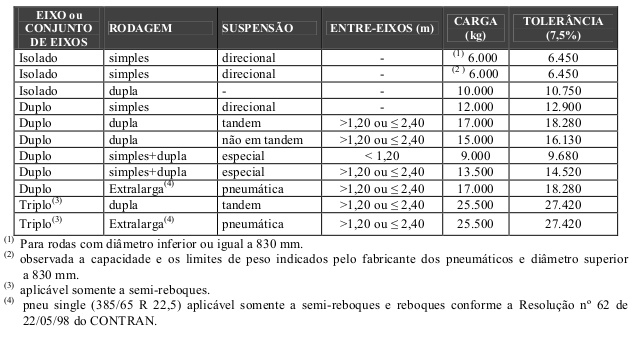
\includegraphics[scale=0.5]{./figuras/tabela-peso-por-eixo.png}
\end{figure}

Os veículos são classificados de acordo com a distribuição dos seus eixos. O \citeonline[p. 15]{tech:dnit-qvf} apresenta uma lista com mais de 150 classificações de veículos, que podem trafegar sem necessidade de um AET. Quando o fabricante especificar um limite inferior ao da tabela apresentada pelo \citeonline{tech:dnit-qvf}, deve ser considerado o menor valor como referência.

A fiscalização de peso de veículos pesados, em rodovias federias no Brasil, é feita pelos Postos de Pesagem Veicular (PPV) do DNIT e da ANTT, e também pode ser feita através de encaminhamento dos veículos pela Polícia Rodoviária Federal (PRF) a esses postos.

A Figura \ref{fig:ppv} mostra um PPV visto de cima. Nessa imagem é possível identificar uma área maior pavimentada destinada ao patio (B), a sala de controle do PPV (A) e a balança de precisão (C). Na Figura \ref{fig:balanca-precisao} pode ser visto um caminhão passando pela balança de precisão.

\begin{figure}[h!]
  \caption{Posto de Pesagem Veicular (PPV)}
  \label{fig:ppv}
  \centering
    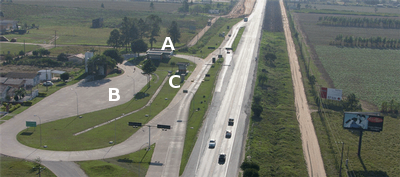
\includegraphics[scale=0.7]{./figuras/ppv_aerea_id.png}
\end{figure}

\begin{figure}[h!]
  \caption{Balança de precisão}
  \label{fig:balanca-precisao}
  \centering
    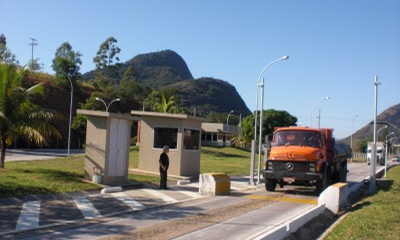
\includegraphics[scale=0.7]{./figuras/balanca-de-precisao.jpg}
\end{figure}

Quando o peso verificado for igual ou inferior ao PBT ou PBTC (peso bruto total combinado) estabelecido para o veículo, acrescido da tolerância de 5\%, porém ocorrer excesso de peso em algum dos eixos, ou conjunto de eixos, acrescido de 5\%, será aplicado a multa sobre a parcela que exceder essa tolerância. Além disso, o veículo somente poderá seguir viagem quando a carga for ser remanejada ou ser feito o seu transbordo, de modo a eliminar os excessos de carga por eixo \cite{tech:dnit-ppv-guia-pratico-operacao}.

\section{Sistemas de pesagem de veículos}\label{sec:ppv-sistemas}
A pesagem de veículos é realizada por sistemas compostos de equipamentos e programas computacionais. Na lista de componentes destes sistemas podem ser encontrados: placas de aquisição, amplificador de carga, sensores, computadores, câmeras de reconhecimento automático de placas de identificação veicular (ALPR), circuitos indutivos, etc. 

Os programas de computador devem ser capazes de processar em tempo hábil informações como: velocidade, distância entre eixos, grupos de eixos, peso por eixo, peso por grupo de eixo, peso bruto total (PBT), classificação do veículo e excesso de peso por eixo e por PBT. Além dessas informações o sistema precisa vinculá-las à identificação do veículo, seja por câmeras ALPR ou seja através de entrada manual dessa informação no sistema.

Além da questão de equipamentos e programas computacionais, é importante salientar a importância das condições estruturais do pavimento para a acurácia dos sistemas de pesagem.

Na Figura \ref{fig:sistema-hswim} é possível visualizar um computador conectado a duas placas de aquisição (equipamentos brancos no centro da imagem) e a um amplificador de carga (equipamento azul no canto superior esquerdo). Essa figura, extraída da revista PÓS-WIM do 1\grad Seminário Internacional de Pesagem em Movimento, é de de um sistema de pesagem em alta velocidade localizada na cidade de Araranguá/SC.

\begin{figure}[h!]
  \caption{Sistema para pesagem em movimento em alta velocidade \cite{magazine:pos-wim-1}}
  \label{fig:sistema-hswim}
  \centering
    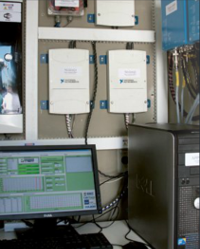
\includegraphics[scale=1]{./figuras/abrigo-pista-experimental.png}
\end{figure}

Nos PPVs sob jurisdição do DNIT, destacam-se duas tecnologias de sensores: \textit{bending plates} e célula de cargas hidráulicas(ou \textit{hydraulic load-cell}).

A tecnologia \textit{bending plate} funciona através de placas metálicas providas de sensores do tipo \textit{strain gages}, localizados na parte de baixo de uma cava especial no pavimento, geralmente com dimensões de 70,0 x 40,0 cm e posicionadas transversalmente ao fluxo de veículos, perfeitamente niveladas com o piso \cite{article:albanorevisando}.

Os sistemas que operam com células de carga hidráulicas (\textit{hydraulic load-cel}), em geral, operam transferindo a carga da roda aplicada sobre a plataforma de pesagem sobre um ou mais cilindros hidráulicos contendo óleo especial, a alteração na pressão hidráulica provocada é correlacionada com a carga por eixo \cite{article:albanorevisando}.

Em \cite[p. 8]{ref:zhang2007evaluating}, é apresentado pelos autores uma tabela comparativa entre os tipos de sensores utilizados na pesagem de veículos. Observa-se que os sensores do tipo \textit{bending plate} são mais baratos que os de células de carga, porém, este último, apresenta acurácia maior dentro de 95\% de confiança (ver Figura \ref{fig:tabela-comparacao-sensores}).

\begin{figure}[h!]
  \caption{Comparação entre sensores de pesagem \cite{ref:zhang2007evaluating}}
  \label{fig:tabela-comparacao-sensores}
  \centering
    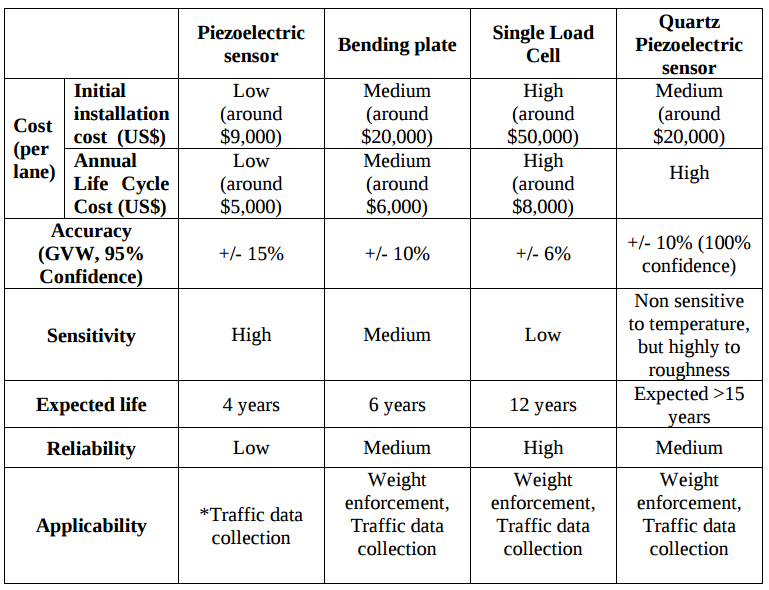
\includegraphics[scale=0.4]{./figuras/tabela-comparacao-siwim.png}
\end{figure}

% ------------------------------------------------------------

\chapter{Algoritmos de apoio à pesgem em movimento}\label{algoritmos}
Um sistema computacional para a pesagem de veículos em movimento consiste essencialmente de:

\begin{itemize}
\item Aquisição de sinal dos sensores de peso (balança);
\item Segmentação sinal (para cortar o respectivo sinal para o caminhão medido);
\item Processamento digital de sinal;
\item Cálculos (velocidade, número de eixos, conjuntos de eixos, distância entre eixos, o peso total, o peso por eixo, peso grupo de eixos, comprimento);
\item Classificação veicular;
\item Calibração;
\item Reconhecimento de placa de identificação veicular;
\item Detecção de infracções;
\end{itemize}

O sistema deve ser rápido e robusto para processar todas essas informações em um tempo que seja suficiente para sinalizar e indicar ao usuário da pista que seu veículo deve ser direcionado a um posto de pesagem. \textit{Python} não é uma língua conhecida por ter um elevado nível de desempenho, por isso é necessária a utilização de bibliotecas e métodos para melhorar as suas capacidades de processamento.

Com base nos resultados da pesagem, classificação e reconhecimento de placa de identificação do veículo, é possível saber se o veículo está com sobrepeso e, em caso afirmativo, é possível vincular a infração à identidade do veículo.

A construção dos algoritmos serão apoiadas pelas bibliotecas computacionais: \textit{numpy, scipy, pandas, sqlalchemy, statsmodels, numba, scikit-learn, pydaqmx, bokeh, ipython, jupyter}.

\section{Aquisição de dados}\label{algoritmos-daq}
O módulo de aquisição de dados é responsável por adquirir dado provenientes da placa de aquisição, que está conectada aos sensores de peso. Para a elaboração dessa seção, foi utilizada como referência a placa de aquisição \textit{DAQmx} da empresa \textit{National Instruments (NI)}. Para comunicar-se com este tipo de placa, será utilizada como apoio a biblioteca computacional \textit{PyDAQmx} que é uma interface completa para os controladores da placa.

Após a aquisição do sinal dos sensores, o sistema armazena estes dados em uma memória circular, dentro de um processo paralelo, onde são analisados com o objetivo de encontrar um sinal de um veículo (segmentação). Este processo foi construído de maneira muito simples, onde o programa aguarda que o sinal proveniente de um circuito indutivo e, quando acionado, segmenta o sinal com dados respectivos aos 3 segundos seguintes.

%==========================================
% CARACTERIZAÇÃO DA PLACA DE AQUISIÇÃO
%==========================================

\subsection{Características da Placa de Aquisição}\label{placa-aquisicao}

A National Instruments (NI) é uma empresa produtora de equipamento de teste automatizado e software de instrumentação virtual com aplicações comuns de aquisição de dados, controle de instrumentos e visão artificial.

O sistema de Pesagem em Movimento (\textbf{WIM}) está estruturado em: 
\begin{itemize}
  \item Aquisição dos sinais transmitidos através dos sensores piezoelétricos e captados pela placa de aquisição \textbf{NI USB DAQmx};
  \item Processamento do sinal (segmentação, filtro, detecção de pico, etc);
  \item Cálculos para obtenção do peso do caminhão
  \item Armazenamento dos dados e informações coletados.
\end{itemize}

A placa utilizada no projeto \textbf{WIM} é a \textbf{NI USB DAQmx 6251} para os sensores piezoelétricos de quartzo. Para trabalhar com essa placa é necessário utilizar os componentes disponibilizados pela NI. No site da fabricante é possível verificar as placas e os componentes e sistemas operacionais compatíveis \cite{nidamx-portable-devices}. 

Para parametrizar algumas funções da biblioteca \textbf{NIDAQmx} é importante ter conhecimento algumas especificações da placa \textbf{NIDAQ USB 6251}.

\begin{description}
  \item Taxa de Amostragem (Sampling rate):
  \begin{itemize}
    \item 1.00 MS/s (multi canais)
    \item Tempo de acurácia 50 ppm de taxa de amostra
    \item Tempo de resolução 50 ns
  \end{itemize}
\end{description}

\begin{description}
  \item Buffer:
  \begin{itemize}
    \item Tamanho de Entrada FIFO: 4095
    \item Memória de lista capturada: 4095 entradas
  \end{itemize}
\end{description}

%==========================================
% MÉTODOS PARA AQUISIÇÃO DE DADOS
%==========================================

\subsection{Métodos para Aquisição de Dados}\label{metodo-aquisicao}

A aquisição de dados é basicamente estruturada em sensores, placa de aquisição e processamento dos sinais recebidos. O processamento dos sinais é feito através da biblioteca \textbf{NIDAQmx} (bibliotecas escritas em \textbf{C/C++}) e são utilizadas em \textbf{Python} através do \textbf{PyDAQmx}.

A aquisição de dados com a biblioteca \textbf{NIDAQmx} pode ser: contínua, finita ou \textit{Hardware Timed Single Point}. Cada modo possui características específicas e está apresentada abaixo uma breve descrição de cada um:

\begin{description}
  \item Aquisição Contínua
    \begin{itemize}
      \item Trabalha internamente com \textit{buffer} circular \cite{nidaqmx-faq};
    \end{itemize}
  \item Aquisição Finita
    \begin{itemize}
      \item Em casos gerais deve-se usar o método \textit{WaitUntilTaskDone} com método em modo finito de medições e gerações antes de solicitar a parada da tarefa \cite{nidaqmx-using-wait-until-done}.
    \end{itemize}
  \item Aquisição \textit{Hardware Timed Single Point}
    \begin{itemize}
      \item A biblioteca \textbf{NIDAQmx} não cria \textit{buffer} para armazenar os valores obtidos \cite{nidaqmx-hwtspsamplemode}.
      \item Para a Placa \textbf{NIDAQ USB 6251} o modo de aquisição \textit{Hardware Timed Single Point} não funcionou, retornando o erro (-2000077).
    \end{itemize}
\end{description} 

O desempenho e a qualidade dos dados medidos vai depender da estratégia adotada para fazer a aquisição e os parâmetros definidos nos métodos.

Sobre a taxa de amostragem, em geral, a \textbf{NI} recomenda utilizar o teorema de \textbf{Nyquist} para definir o valor da taxa de amostragem que diz que um sinal deve ser amostrado a uma taxa maior que duas vezes a componente de maior frequência de interesse no sinal para que essa componente seja capturada \cite{nidaqmx-conceitos-basicos-amostragem-analogica}.

Porém, para o sistema de pesagem em movimento a fabricante dos sensores de aquisição desenvolveu um cálculo para definir a taxa de amostragem \cite[p. 9]{kistler2004installation}.

\begin{equation}
Taxa\ de\ Amostragem = \frac{velocidade(m/s)\ \times \ m\acute{\imath}nimo\ de\ pontos\ medidos\ (por\ curva)}{largura\ da\ impressão\ do\ pneu}
\end{equation}

Através de seus estudos a fabricante chegou a uma taxa de amostragem recomendada de \textbf{2 MHz} \cite[p. 9]{kistler-instruction-manual}.

A estrutura geral de aquisição com a biblioteca \textbf{NIDAQmx} é: 
\begin{enumerate}
\item Criação da tarefa (\textit{Task Configuration/Control});
\item Definição do método de Amostragem (\textit{Timing});
\item Início da tarefa (\textit{Task Configuration/Control});
\item Leitura de sinal (\textit{Read Functions} ou \textit{Events Callback});
\item Fim da tarefa (\textit{Task Configuration/Control});
\end{enumerate}

Para visualizar a lista completa das funções disponíveis na biblioteca \textbf{NIDAQmx} acesse o site da \textbf{NI} \cite{nidaqmx-c-reference}.

%==========================================
% ESTRATÉGIA DE AQUISIÇÃO
%==========================================-

\subsection{Estratégia de Aquisição de Dados}\label{estrategia-aquisicao}
A estratégia para adquirir os dados vai depender das necessidades e condições de execução do sistema (como por exemplo, memória, processamento, latência, etc). 

A aquisição é definida através de uma tarefa (\textit{Task}) e pode ser configurada para ler 1 ou mais canais de um dispositivo (placa), cada dispositivo necessita de uma tarefa única.

Alguns exemplos de aquisição podem ser encontrados no sítio web do \textbf{PyDAQmx} \cite{pydaqmx}.

A continuação estão listadas algumas das opções para fazer a aquisição de dados com a biblioteca \textbf{NIDAQmx}. 

%==========================================
% ESTRATÉGIA: AQUISIÇÃO CONTÍNUA INICIADA 
% UMA UNICA VEZ
%==========================================

\subsubsection{Aquisição contínua, tarefa iniciada uma única vez}\label{aquisicao-continua}

A biblioteca \textbf{NIDAQmx} pode ser configurada para adquirir em modo contínuo. Nesse modo é iniciada apenas uma vez a tarefa (deve ser criada uma tarefa por dispositivo), a leitura dos sinais é feita dentro de um laço de repetição infinita e é necessário utilizar um comando para aguardar por um tempo determinado suficiente para que o \textit{buffer} interno da biblioteca consiga armazenar a quantidade de amostras definidas para a leitura. A seguir está listada um exemplo com os passos para realizar esse tipo de aquisição:
\begin{enumerate}
  \item Cria tarefa (\textit{CreateTask});
  \item Configura o tempo de amostragem em modo continuo (\textit{DAQmxCfgSampClkTiming});
  \item Inicia a tarefa de aquisição (\textit{DAQmxStartTask});
  \item Inicia um laço de repetição (laço infinito);
  \item Leitura do sinal a cada N amostras(\textit{DAQmxReadAnalogF64});
  \item Calcula o \textit{timestamp} para cada linha de sinal adquirido;
  \item Repete laço infinitamente;
  \item Finaliza a tarefa de aquisição (\textit{DAQmxStopTask})
\end{enumerate}

%==========================================
% ESTRATÉGIA: AQUISIÇÃO CONTÍNUA INICIADA 
% UMA UNICA VEZ, LEITURA ATRAVÉS DE CALLBACK
%==========================================
\subsubsection{Aquisição contínua, tarefa iniciada uma única vez com \textit{callback}}\label{aquisicao-continua-callback}

A biblioteca \textbf{NI DAQmx} permite a configuração de uma função de \textbf{callback} para ser executada automaticamente após a leitura de $N$ número de amostras em cada canal utilizando a aquisição em modo contínua. O \textit{timestamp} deverá ser calculado para cada item da amostra, ou seja, N \textit{timestamps} de intervalo $\Delta t$ (calculado com base na taxa de amostragem). Para que o sistema não encerre durante a espera dos \textit{callbacks} pode ser utilizado o comando \textit{raw\_input} que faz a execução do sistema esperar por um \textit{ENTER} para prosseguir. A continuação segue exemplo de aquisição com \textit{callback}:

\begin{enumerate}
  \item Cria tarefa por dispositivo (\textit{CreateTask});
  \item Configura o tempo de amostragem em modo continuo (\textit{DAQmxCfgSampClkTiming});
  \item Define a aquisição através de \textit{callback} (\textit{RegisterEveryNSamplesEvent e RegisterDoneEvent})
  \item Dentro do método \textit{EveryNCallback} realizar a leitura dos sinais (\textit{DAQmxReadAnalogF64}) e calcular o \textit{timestamp} para cada aquisição da amostragem (para cada N amostras por canal deve ter uma lista com N \textit{timestamps} ($\Delta t$ de acordo com a taxa de amostragem);
  \item Inicia a tarefa de aquisição de cada dispositivo(\textit{DAQmxStartTask});
  \item Aciona comando de interrupção de teclado (\textit{raw\_input}) para não encerrar o processamento do sistema enquanto o sistema faz a aquisição por \textit{callback};
  \item Quando for pressionada a tecla \textit{<ENTER>} finaliza a tarefa de aquisição de cada dispositivo(\textit{DAQmxStopTask}) e encerra a execução do sistema.
\end{enumerate}

%==========================================
% ESTRATÉGIA: AQUISIÇÃO FINITA INICIADA 
% TASK POR CANAL; INICIO, LEITURA e PARADA 
% DA TASK DENTRO DE UM LAÇO DE REPETIÇÃO
%==========================================
\subsubsection{Aquisição de amostragem finita e uma tarefa por canal}\label{aquisicao-finita-loop-infinito}

Para trabalhar com aquisição de amostragem finita deve ser considerado criar uma tarefa para cada canal. A aquisição ficará dentro de um laço infinito e ela será individual para cada canal (inicio de aquisição, leitura e encerramento da aquisição). A leitura deverá retornar apenas uma amostra por vez e por isso não é necessário utilizar o método de \textit{Clock Time Sampling}, o tempo entre cada aquisição deverá ser feita através de um método do tipo \textit{sleep} (tempo de espera). A seguir a ilustração dos passos para a aquisição finita:

\begin{enumerate}
  \item Cria uma tarefa para cada canal(\textit{CreateTask});
  \item Inicia o laço de repetição infinita;
  \item Para cada canal:
    \begin{enumerate}
      \item Inicia a tarefa de aquisição (\textit{DAQmxStartTask});
      \item \textbf{1 amostra} por leitura (\textit{DAQmxReadAnalogF64});
      \item Armazena o valor adquirido junto com o \textit{timestamp} atual do sistema;
      \item Finaliza a tarefa de aquisição (\textit{DAQmxStopTask});
    \end{enumerate}
  \item Repete laço infinitamente a cada X tempo;
\end{enumerate}

%==========================================
% APLICAÇÃO E RESULTADOS
%==========================================
\subsection{Aplicação e Resultados}\label{aplicacao-resultado}
A \textbf{National Instruments}, empresa que fabrica as placas \textbf{NI DAQmx}, disponibiliza um conjunto de aplicativos para auxiliar o desenvolvimento e testes dos dispositivos e bibliotecas criados pela mesma \cite{nidaqmx-cd-9.8}. Entre esses aplicativos encontra-se o \textbf{NI MAX} que permite realizar simulações e testes de aquisição e geração de sinais utilizando parâmetros reais para a configuração da tarefa, como modo de amostragem, tensão máxima, frequência, etc. É possível também criar placas simuladas específicas para a realização dos testes.

%==========================================
% APLICAÇÃO E RESULTADOS - Leitura da Entrada Lógica
%==========================================
\subsubsection{Leitura da Entrada Analógica}
Foram analisadas diferentes opções de leitura para avaliar performance, consumo de memória e consumo de processamento

\begin{table}[htbp]
  \centering
  \begin{footnotesize}
    \begin{tabular}{|p{3cm}|p{2cm}|p{2cm}|p{2cm}|}
      \textbf{Modo de Aquisição} & \textbf{Desempenho} & \textbf{Consumo de memória} & \textbf{Consumo de Processamento} \\ \hline
       Aquisição finita & Baixa & Alto & Alto \\ \hline
       Aquisição contínua com \textit{callback} & Alta & Baixo & Baixo\\ \hline
    \end{tabular}
  \end{footnotesize} 
  \caption{Comparativo entre diferentes modos de aquisição}
  \label{tab:comparativo-aquisição}
\end{table} 


%==========================================
% APLICAÇÃO E RESULTADOS - GERAÇÃO
%==========================================
\subsubsection{Escrita na Saída Analógica}
Através do \textbf{NI MAX} e algoritmos externos foram realizados testes com geração de sinal com as placas \textbf{NI DAQmx 6343 e 6251} simuladas. Os testes com as placas reais \textbf{NI DAQmx 6343}, por sua vez, apresentaram alguns problemas e foi necessário alterar o fluxo do algoritmo para o correto funcionamento da geração. O algoritmo foi desenhado para trabalhar com a geração em modo finito dentro de um laço infinito utilizando os sinais já adquiridos em outras medições para simular a geração de sinais reais.

A estrutura do algoritmo deverá seguir os seguintes passos:

\begin{enumerate}
  \item Criação da tarefa (\textit{DAQmxCreateTask});
  \item Configuração dos canais de saída analógica (\textit{DAQmxCreateAOVoltageChan});
  \item Configuração da amostragem (modo finito) da tarefa (\textit{DAQmxCfgSampClkTiming});
  \item Inicia um laço de repetição infinita;
  \item Caso estiver alguma ação pendente espera a conclusão da tarefa (\textit{DAQmxWaitUntilTaskDone}) e para a tarefa (\textit{DAQmxStopTask});
  \item Envia dados para a saída analógica da placa (\textit{DAQmxWriteAnalogF64});
  \item Repete o laço até o usuário enviar sinal de interrupção;
\end{enumerate}

\begin{lstlisting}[language=Python, caption=Aquisição de dados com PyDAQmx, label={lst:pydaqmx}]
samples_per_channel = 1000
number_of_channels = 1

task = pydaq.Task()

task.CreateAIVoltageChan()

task.CfgSampClkTiming()
total_samples = pydaq.int32()
data_size = samples_per_channel * number_of_channels
data = np.zeros((data_size,), dtype=np.float64)

task.StartTask()

data = task.ReadAnalogF64(
    samples_per_channel,
    10.0,
    pydaq.DAQmx_Val_GroupByChannel,
    data,
    data_size,
    pydaq.byref(total_samples),
    None
)

p = plt.figure(title='DAQ', width=600, height=300)
p.line(np.linspace(0, 3, 15000), data, legend='sensor 1')
plt.show(p)
\end{lstlisting}

\subsection{Uso de datos sintéticos}\label{algoritmos-daq-sintetico}

\begin{lstlisting}[language=Python, caption=Geração de dados sintéticos, label={lst:daq-sintetico}]
df = pd.DataFrame()

sample_rate = 2000
total_seconds = 3.0

# analog channel 1
df['a1'] = gen_synthetic_analog_data(
    sample_rate=sample_rate, total_seconds=total_seconds, 
    time_delay=0.7, noise_p=10
)

# analog channel 2
df['a2'] = gen_synthetic_analog_data(
    sample_rate=sample_rate, total_seconds=total_seconds, 
    time_delay=1.0, noise_p=10
)

# digital loop
df['d1'] = gen_synthetic_digital_data(
    sample_rate=sample_rate, total_seconds=total_seconds, 
    time_delay=0.8
)

# ploteo
p = charts.Line(
    df, title="Datos de los sensores", 
    xlabel='Segundos (s)', ylabel='Tensao (V)', 
    width=700, height=400, legend=True
)
plt.show(p)
\end{lstlisting}

% --------------------
\section{Armazenamento de dados}\label{algoritmos-armazenamento}

Após segmentado, os dados brutos são armazenados na base de dados. Isso faz com que seja possível mudar os métodos de cálculo de parâmetros ou de calibração, o que torna possível analisar os métodos utilizados.
Em todos os métodos de cálculos e funções do sistema, o padrão para os conjuntos de dados é do tipo \textit{pandas.DataFrame}. Isto é usado desde o tempo de leitura no banco de dados, juntamente com \textit{sqlalchemy}, mesmo nos cálculos, plotagem e gravação de arquivos de banco de dados ou \textit{CSV}. Os mecanismos \textit{pandas.DataFrame} fornece para a manipulação muito semelhantes aos usados em dados de linguagem \textit{R}.

\begin{lstlisting}[language=Python, caption=Armazenamento e consulta na base de datos, label={lst:bd}]
# Connect to the database
DATABASE = {
    'host': 'localhost',
    'database': 'pywim',
    'port': '5432',
    'user': 'pywim',
    'password': 'pywim'
}

conn = psycopg2.connect(**DATABASE)

engine = sqlalchemy.create_engine(
    'postgresql+psycopg2://',
    creator=lambda: conn
)

# creates acquisition data
cur = conn.cursor()
cur.execute(
    'INSERT INTO wim.acquisition (id, date_time) ' +
    'VALUES (DEFAULT, %s) RETURNING id', (datetime.datetime.now(),)
)

acq_id = cur.fetchone()[0]

conn.commit()
cur.close()

df_data = df.copy()
df_data['acquisition'] = acq_id
df_data['time_seconds'] = df_data.index
df_data.rename(
    columns={
        'a1': 'sensor1', 'a2': 'sensor2', 'd1': 'inductive_loop'
    }, inplace=True
)

df_data.to_sql(
    'acquisition_data', con=engine, 
    schema='wim', if_exists='append', index=False
)

conn.commit()

# select acquisition data from database
df_data = pd.read_sql_query(
    '''
    SELECT * FROM wim.acquisition_data
    WHERE acquisition=%s
    ''' % acq_id, con=engine,
    index_col='time_seconds'
)

df_data.drop('acquisition', axis=1, inplace=True)

# ploteo
p = charts.Line(
    df_data[['sensor1', 'sensor2', 'inductive_loop']], 
    title="Datos de los sensores", 
    xlabel='Segundos (s)', ylabel='Tensao (V)', 
    width=700, height=400, legend=True
)
plt.show(p)

\end{lstlisting}
% --------------------
\section{Processamento digital de sinal}\label{algoritmos-dsp}



% --------------------
\section{Cálculos}\label{algoritmos-calculos}


% --------------------
\section{Classificação Veicular}\label{algoritmos-classificacao}


% --------------------
\section{Calibração dos cálculos de pesagem}\label{algoritmos-calibracao}


% --------------------
\section{Reconhecimento automático de placas de identificação veicular}\label{algoritmos-alpr}

% ------------------------------------------------------------

\chapter{Conclusão}\label{conclusao}

Os efeitos causados por caminhões trafegando acima do limite de carga podem ser sentidos pela deterioração prematuras do pavimento e pelos acidentes ocorridos nas rodovias.

Nesse contexto, é evidente a importância da fiscalização, de modo efetiva, para coibir o tráfego de veículos co sobrepeso.

O sobrepeso e má distribuição da carga poderá prejudicar o condutor em questões de estabilidade, inclinação da iluminação, consumo excessivo de combustível, desgaste desnecessário de peças, custos (multas) e tempo (remanejamento ou transbordo).

Atualmente, no Brasil, os sistemas ainda precisam ser aprimorados para alcançar as condições para a fiscalização e autuação direta. Esse tipo de abordagem permite fiscalizar todos veículos pesados que passarem pela via, de maneira transparente e sem interferir na viagem dos veículos que transitam abaixo dos limites estabelecidos por lei.


\bibliographystyle{ufsc-alf}
\bibliography{bibliografia}

%--------------------------------------------------------
% Elementos pós-textuais

\apendice
\chapter{Teste Apęndice}
\section{Entrevista com o pesquisador Helio Goltsman}

Helio Goltsman é engenheiro pesquisador graduado pela PUC-RJ, especializou-se em planejamento de transportes urbanos pela \textit{Massachusetts Institute of Technology - MIT}. Também foi um dos pioneiros da área de pesagem de veículos pesados no Brasil, atuando desde 1974 nesse tema.

Questionário:

\begin{enumerate}
\item Quais entidades autorizadas a realizar a fiscalização de veículos de carga em rodovias federais?\\
R: Nas rodovias federias, estão autorizados o DNIT e a ANTT. A Polícia Rodoviária Federal (PRF) tem autoridade também de realizar blitz para fiscalizar o peso dos veículos pesados e, se necessário, encaminhá-los ao Posto de Pesagem Veicular (PPV) mais próximo.

\item Quais são os maiores problemas encontrados no passado referentes à pesagem de veículos pesados?\\
R: Havia muito problemas com a pesagem móvel. Esse tipo de pesagem era realizada com uma balança móvel compartilhada com mais de uma localização, tendo que ser transladada diariamente para diferentes localidades. A operação de retirar o equipamento de um posto para instalá-lo em outro, consumia muito tempo, diminuindo o tempo de operação da fiscalização.

\item Quais são os maiores problemas encontrados na atualidade referentes pesagem de veículos pesados?\\
R: Um dos problemas encontrados hoje está relacionado ao alto custo para criar e manter um PPV. Hoje, todos os postos de pesagem federais estão inoperantes por determinação da justiça do trabalho por entender que a operação dos mesmos está terceirizada. 

Outro problema está relacionado com os sistemas de pesagem de pré-seleção. 
Estes sistemas possuem uma margem de erro muito alta, acarretando no encaminhamento de muitos veículos sem sobrepeso para o sistema de pesagem de precisão (baixa velocidade). De acordo com as análises dos dados coletados das pesagens nos postos de pesagem, dos 80\% dos veículos encaminhados à balança de precisão, somente 10\% estão realmente com sobrepeso.

\item Quais são as perspectivas de futuro para a pesagem de veículos pesados?\\
R: O objetivo final é a fiscalização e autuação na velocidade diretriz da via, igual é feito para o controle de velocidade, sem ter o posto de pesagem. Para atender este objetivo, muitas pesquisas ainda deverão ser realizadas ao longo de algumas décadas. Essa questão envolve replanejamento em relação a legislação vigente, ao modo como é feita a pesagem, devem ser estudados tópicos como, por exemplo, a localização das áreas de descarga e descanso. O próximo passo para alcançar esses objetivos será a implantação dos Postos Integrados Automatizados de Fiscalização (PIAFs), onde a pré-seleção na rodovia será feita na velocidade normal da via e, somente quando for constatada a infração, o veículo será encaminhado à balança de precisão do PPV.

\end{enumerate}

\anexo
\chapter{Teste Anexo}
conteúdo do anexo

\end{document}
%%%%%%%%%%%%%%%%%%%%%%%%%%%%%%%%%%%%%%%%%%%%%%%%%%%%%%%%%%%%%%%%%%%%%%%
% Fim do documento                                
%%%%%%%%%%%%%%%%%%%%%%%%%%%%%%%%%%%%%%%%%%%%%%%%%%%%%%%%%%%%%%%%%%%%%%%



%%%%%%%%%%%%%%%%%%%%%%%%%%%%%%%%%%%%%%%%%%%%%%%%%%%%%%%%%%%%%%%%%%%%%%%
% Identificadores do trabalho
% Usados para preencher os elementos pré-textuais
%%%%%%%%%%%%%%%%%%%%%%%%%%%%%%%%%%%%%%%%%%%%%%%%%%%%%%%%%%%%%%%%%%%%%%%

%----------------------------------------------------------------------
% Só preencher se năo for a UFSC - Se for uma instituiçăo "masculina",
% como um Instituto Federal, usar o parâmetro opcional [] - v. exemplo
%
%\instituicao[o]{Instituto Federal do Rio Grande do Sul}

%----------------------------------------------------------------------
% Só preencher se năo for o departamento de Eng. Mecânica - o que deve 
% ser quase que certo. Se for um departamento "feminino", usar o
% parâmetro opcional [] - v. exemplo
%
%\departamento[a]{Faculdade de Cięncias do Mar}

%----------------------------------------------------------------------
% Só preencher se năo for o POSMEC - o que deve ser quase que certo.
% Se for um curso "feminino", usar o parâmetro opcional [] - v. exemplo
%
%\curso[a]{Atividade de Extensăo em Corte e Costura}

%----------------------------------------------------------------------
% Só preencher se năo for tese
% Se for um documento diferente de tese, dissertaçăo, tcc, monografia
% ou relatório, indicar no parâmetro opcional o gęnero - v. exemplo
%
%\documento[o]{Laudo}

%----------------------------------------------------------------------
% Título é obrigatório, mas subtítulo é opcional
%
%\titulo{Elaboraçăo de documentos para a BU/UFSC}
%\subtitulo{Estilo \LaTeX~ Padrăo}

%----------------------------------------------------------------------
% Autor é obrigatório. Năo se atreva a năo incluir ou vai ter surpresa
%
%\autor{Roberto Simoni, Carlos R Rocha}

%----------------------------------------------------------------------
%
% Só preencher se năo for Doutor em Engenharia Mecânica
%\grau{Descomentar se năo for Doutor em Engenharia Mecânica}

%----------------------------------------------------------------------
% Só preencher se năo for Florianópolis
%
%\local{Simcity}

%----------------------------------------------------------------------
% Data deve ter as tręs partes entre chaves
%
%\data{01}{julho}{2010}

%----------------------------------------------------------------------
% Orientador é obrigatório. Coorientador é opcional
% Se o título for diferente (orientadora), indicar como no exemplo
%
%\orientador[Orientadora]{Profa. Dra. Fulana}
%\coorientador{Prof. Dr. Beltrano}

%----------------------------------------------------------------------
% Coordenador do programa é obrigatório
% Se o título for diferente (coordenadora), indicar como no exemplo
%
%\coordenador[Coordenadora]{Profa. Senhora, Dra. Eng.}

%----------------------------------------------------------------------
% Banca - Pode ter até 7 membros além de orientador e co-orientador
% Se estes săo parte da banca, devem ser adicionados com os comandos
% \orientadornabanca{sim} e \coorientadornabanca{sim}
% do contrário, eles aparecerăo antes da designaçăo da banca
% O MembroA da banca é por definiçăo o seu presidente
% O numero total de membros na defesa decide se a folha de aprovaçăo
% deverá ser duplicada. Se passar de 4, uma folha adicional de assinaturas
% será gerada
%
%\numerodemembrosnabanca{4} % Isso decide se haverá uma folha adicional
%\orientadornabanca{sim} % Se faz parte da banca definir como sim
%\coorientadornabanca{sim} % Se faz parte da banca definir como sim
%\bancaMembroA{Prof. Presidente da banca} %Nome do presidente da banca
%\bancaMembroB{Prof. segundo membro}      % Nome do membro da Banca
%\bancaMembroC{Prof. terceiro membro}     % Nome do membro da Banca
%\bancaMembroD{Prof. quarto membro}       % Nome do membro da Banca
%\bancaMembroE{Prof. quinto membro}       % Nome do membro da Banca
%\bancaMembroF{Prof. sexto membro}        % Nome do membro da Banca
%\bancaMembroG{Prof. sétimo membro}       % Nome do membro da Banca

%----------------------------------------------------------------------
% Firulas opcionais - Dedicatória, Agradecimento e Epígrafe
%
% \dedicatoria{Dedicatória para alguem}
% \agradecimento{Agradecimentos, se for o caso...blabla blablablabla blabla ipsum loren e a sophia também blab ablablabl ablbalbalblab lablablbalb lab la}
% \epigrafe{Um bonito pensamento ou citaçăo, se for o caso}{autor do pensamento}

%----------------------------------------------------------------------
% Resumo e abstract - É só definir como mostra o exemplo abaixo
% 
% \textoResumo {Aqui é redigido o resumo do documento...  blabla blablablabla blabla ipsum loren e a sophia também blab ablablabl ablbalbalblab lablablbalb lab lab lab labl a blab lablablab la blab alballbalba lba lba }
% \palavrasChave {chave 1. chave 2. ... chave n.}
% 
% \textAbstract {Here is written the abstract of the document}
% \keywords {key 1. key 2. ... key n.}
